\documentclass[aspectratio=169,10pt]{beamer}

\usepackage[T1]{fontenc}
\usepackage{lmodern}
\usepackage{booktabs}
\usepackage{tabularx}
\usepackage{tikz}
\usetikzlibrary{arrows.meta,positioning,fit,backgrounds}

\definecolor{Forest}{HTML}{153C32}
\definecolor{Mint}{HTML}{C9F0DC}
\definecolor{Cream}{HTML}{F8F6EF}
\definecolor{Rust}{HTML}{B65738}
\definecolor{Muted}{HTML}{64706C}

\setbeamercolor{normal text}{fg=Forest,bg=Cream}
\setbeamercolor{structure}{fg=Forest}
\setbeamercolor{frametitle}{fg=Forest,bg=Cream}
\setbeamercolor{title}{fg=Forest}
\setbeamercolor{subtitle}{fg=Muted}
\setbeamercolor{block title}{fg=Forest,bg=Mint}
\setbeamercolor{block body}{fg=Forest,bg=Mint!32!Cream}
\setbeamercolor{alerted text}{fg=Rust}
\setbeamertemplate{navigation symbols}{}
\setbeamertemplate{itemize item}{\color{Rust}$\blacktriangleright$}
\setbeamertemplate{itemize subitem}{\color{Forest}$\bullet$}
\setbeamertemplate{footline}{%
  \leavevmode\hbox{%
    \begin{beamercolorbox}[wd=.82\paperwidth,ht=2.6ex,dp=1.1ex,leftskip=1em]{author in head/foot}%
      \color{Muted}\scriptsize Digital Professor: interaction and evidence integration
    \end{beamercolorbox}%
    \begin{beamercolorbox}[wd=.18\paperwidth,ht=2.6ex,dp=1.1ex,rightskip=1em plus1fil]{date in head/foot}%
      \color{Muted}\scriptsize\hfill\insertframenumber/\inserttotalframenumber
    \end{beamercolorbox}}}
\setbeamertemplate{frametitle}{\vspace{.35em}\insertframetitle\par\vspace{.15em}\hrule height .4pt}

\title{Interaction Integration Module Update}
\subtitle{Inputs, functions, outputs, and downstream handoffs}
\author{Jonathan Ma}
\institute{Entagile}
\date{October 2026}

\begin{document}

\begin{frame}[plain]
  \vfill
  {\usebeamerfont{title}\color{Forest}\LARGE\inserttitle\par}
  \vspace{.5em}
  {\color{Muted}\large\insertsubtitle\par}
  \vspace{1.5em}
  {\color{Rust}\rule{2.2cm}{2pt}}\par
  \vspace{1.2em}
  {\small\insertauthor\hfill\insertdate}
  \vfill
\end{frame}

\begin{frame}{Where the interaction module fits}
\centering
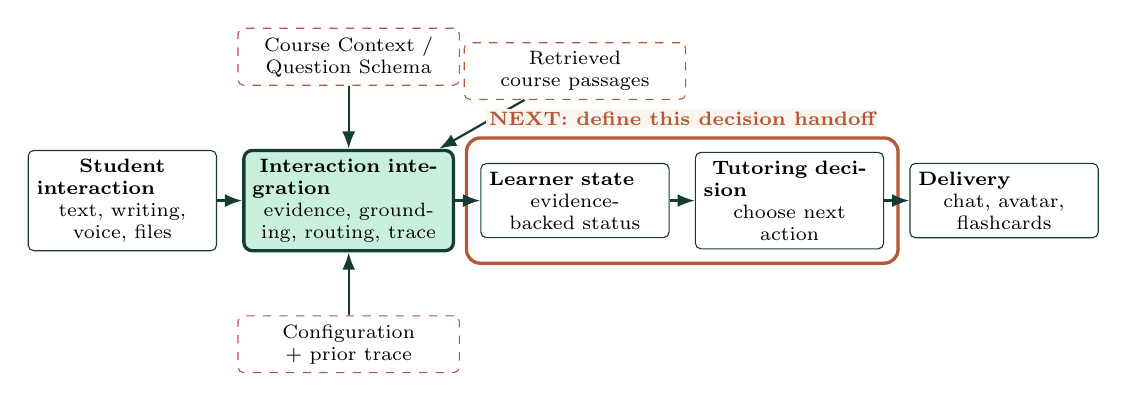
\begin{tikzpicture}[
  node distance=.45cm and .32cm,
  box/.style={draw=Forest,rounded corners=2pt,fill=white,align=center,text width=2.18cm,minimum height=.88cm,inner sep=3pt,font=\scriptsize},
  focus/.style={draw=Forest,very thick,rounded corners=3pt,fill=Mint,align=center,text width=2.45cm,minimum height=1.0cm,inner sep=3pt,font=\scriptsize},
  support/.style={draw=Rust,dashed,rounded corners=2pt,fill=white,align=center,text width=2.6cm,minimum height=.72cm,inner sep=3pt,font=\scriptsize},
  arrow/.style={-{Latex[length=2.2mm]},thick,draw=Forest}]
\node[box] (student) {\textbf{Student interaction}\newline text, writing, voice, files};
\node[focus,right=of student] (integration) {\textbf{Interaction integration}\newline evidence, grounding, routing, trace};
\node[box,right=of integration] (state) {\textbf{Learner state}\newline evidence-backed status};
\node[box,right=of state] (decision) {\textbf{Tutoring decision}\newline choose next action};
\node[box,right=of decision] (delivery) {\textbf{Delivery}\newline chat, avatar, flashcards};
\node[support,above=8mm of integration] (course) {Course Context / Question Schema};
\node[support,above=8mm of state] (rag) {Retrieved course passages};
\node[support,below=8mm of integration] (config) {Configuration + prior trace};
\draw[arrow] (student)--(integration);
\draw[arrow] (integration)--(state);
\draw[arrow] (state)--(decision);
\draw[arrow] (decision)--(delivery);
\draw[arrow] (course)--(integration);
\draw[arrow] (rag)--(integration);
\draw[arrow] (config)--(integration);
\begin{scope}[on background layer]
  \node[draw=Rust,very thick,rounded corners=5pt,fit=(state)(decision),inner sep=5pt] (nextfocus) {};
\end{scope}
\node[above=1mm of nextfocus.north,font=\scriptsize\bfseries,text=Rust,fill=Cream,inner sep=1pt] {NEXT: define this decision handoff};
\end{tikzpicture}
\vspace{.65em}
\textbf{My module is the bridge:} it converts student interaction into trusted evidence and moves that evidence, with its context, through the tutoring loop.
\end{frame}

\begin{frame}{What comes in}
\begin{columns}[T,onlytextwidth]
\column{.48\textwidth}
\begin{block}{Student-side inputs}
\begin{itemize}
\item Text, equations, handwriting, voice, images, or files
\item Recognized content and possible alternatives
\item Student corrections, explanations, and uncertainty
\item Session, question, and turn identity
\end{itemize}
\end{block}
\column{.49\textwidth}
\begin{block}{System-side inputs}
\begin{itemize}
\item Course Context and Question Schema
\item Retrieved passages and page citations
\item Previous learner state and prior tutoring action
\item Tutoring rules and delivery options
\end{itemize}
\end{block}
\end{columns}
\vspace{.45em}
\centering
\textbf{Key rule:} preserve where every item came from so later decisions can be explained and checked.
\end{frame}

\begin{frame}{What the module does}
\begin{columns}[T,onlytextwidth]
\column{.48\textwidth}
\begin{block}{1. Understand the submission}
\begin{enumerate}
\item Identify the input type
\item Run the appropriate recognition tool
\item Ask the student about meaning-changing ambiguity
\item Capture work, answer, explanation, and uncertainty
\end{enumerate}
\end{block}
\column{.49\textwidth}
\begin{block}{2. Prepare and route evidence}
\begin{enumerate}
\item Link the submission to its question and prior help
\item Request supporting course material
\item Validate the evidence record
\item Send it to the learner-state component
\item Record the resulting action and response
\end{enumerate}
\end{block}
\end{columns}
\vspace{.4em}
\centering
\textbf{Boundary:} this module prepares and routes evidence; the downstream components interpret it and choose the tutoring action.
\end{frame}

\begin{frame}{What goes out --- and where it goes}
\small
\begin{tabularx}{\textwidth}{@{}p{0.23\textwidth}p{0.28\textwidth}X@{}}
\toprule
\textbf{Output} & \textbf{Receiver} & \textbf{Purpose} \\
\midrule
Retrieval request & Course Knowledge/RAG & Find relevant course passages and citations. \\
\addlinespace
Student Evidence & Learner State & Determine what the student has demonstrated or still needs. \\
\addlinespace
Grounded turn context & Tutoring Decision & Choose a question, hint, explanation, retry, or reassessment. \\
\addlinespace
Session context & Tutoring Delivery & Present the chosen action through chat, avatar, or another channel. \\
\addlinespace
Interaction trace & Persistent State & Preserve the sequence for continuity and later review. \\
\bottomrule
\end{tabularx}
\vspace{.45em}
\begin{block}{Common contract}
Each handoff includes identity, source, validation status, and the context version used to create it.
\end{block}
\end{frame}

\begin{frame}{A tutoring turn from start to finish}
\centering
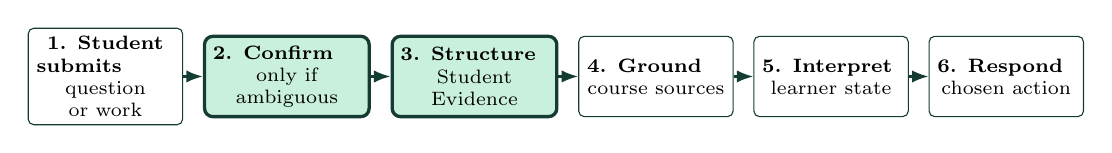
\begin{tikzpicture}[
  node distance=.25cm,
  box/.style={draw=Forest,rounded corners=2pt,fill=white,align=center,text width=1.75cm,minimum height=1.02cm,inner sep=3pt,font=\scriptsize},
  focus/.style={draw=Forest,very thick,rounded corners=3pt,fill=Mint,align=center,text width=1.88cm,minimum height=1.02cm,inner sep=3pt,font=\scriptsize},
  arrow/.style={-{Latex[length=2.1mm]},thick,draw=Forest}]
\node[box] (submit) {\textbf{1. Student submits}\newline question or work};
\node[focus,right=of submit] (confirm) {\textbf{2. Confirm}\newline only if ambiguous};
\node[focus,right=of confirm] (evidence) {\textbf{3. Structure}\newline Student Evidence};
\node[box,right=of evidence] (ground) {\textbf{4. Ground}\newline course sources};
\node[box,right=of ground] (state) {\textbf{5. Interpret}\newline learner state};
\node[box,right=of state] (action) {\textbf{6. Respond}\newline chosen action};
\draw[arrow] (submit)--(confirm);\draw[arrow] (confirm)--(evidence);\draw[arrow] (evidence)--(ground);\draw[arrow] (ground)--(state);\draw[arrow] (state)--(action);
\end{tikzpicture}
\vspace{.7em}
\begin{columns}[T,onlytextwidth]
\column{.48\textwidth}
\begin{block}{The record grows}
The system keeps the original submission, confirmed interpretation, sources, state change, action, and response as one linked history.
\end{block}
\column{.49\textwidth}
\begin{block}{The loop continues}
The student's next response creates new evidence linked to the earlier attempt and intervention. It does not overwrite either one.
\end{block}
\end{columns}
\end{frame}

\begin{frame}{What we need to define next}
\begin{columns}[T,onlytextwidth]
\column{.48\textwidth}
\begin{block}{Primary focus}
\begin{itemize}
\item What Learner State must contain
\item How evidence changes that state
\item What Tutoring Decision receives
\item How it selects and explains an action
\end{itemize}
\end{block}
\column{.49\textwidth}
\begin{block}{Immediate work}
\begin{itemize}
\item Walk through one turn with all module owners
\item Resolve missing or duplicated ownership
\item Agree on minimum handoff fields and failure states
\item Freeze interface version 0.1
\end{itemize}
\end{block}
\end{columns}
\vspace{.45em}
\centering
\textbf{Near-term result:} a clear, reviewable contract from Student Evidence to Learner State to Tutoring Decision.
\end{frame}

\end{document}
